%%%%%%%%%%%%%%%%%%%%%%%%%%%%%%%%%%%%%%%%%%%%%%%%%%%%%%%%%%%%%%%%%%%%%%
% Problem statement
\begin{statement}[
  problempoints=110,
  timelimit=2 sekunde,
  memorylimit=256 MiB,
]{Holding}

\setlength\intextsep{-0.1cm}
\begin{wrapfigure}[9]{r}{0.17\textwidth}
\centering
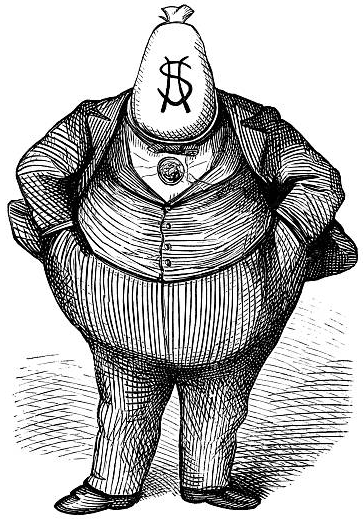
\includegraphics[width=0.17\textwidth]{img/holding.png}
\end{wrapfigure}

Teški su se oblaci nadvili nad Ivičin Holding, skupinu od $N$ tvrtki koje su u
njegovom vlasništvu. Svaka od tih tvrtki je u dugovima i upravo zbog dugova
država je poslala odvjetnike da Ivici uzmu sve što ima. Ivica je, kako
ekskluzivno doznajemo, uspio namoliti državu da mu ipak ostavi neke tvrtke.
Koje? Saznali smo i to.

Odvjetnici su na stol nanizali vlasničke papire $N$ Ivičinih tvrtki. Dug prve
tvrtke u nizu papira je $A_1$, druge $A_2$, \dots i zadnje u nizu $A_N$.
Ivica je dogovorio s državom da mu ostavi u vlasništvu tvrtke s dugovima
$A_L$, $A_{L+1}$, \dots , $A_R$, gdje $L$ i $R$ predstavljaju pozicije u nizu
papira na stolu. Na sreću po Ivicu, odvjetnici su potkupljivi. Istina, neće
dozvoliti da Ivica uzme neki drugi podniz dugova osim onoga dogovorenog
(između $L$-te i $R$-te pozicije u nizu papira), ali kažu da će mu rado
zamijeniti bilo koja dva vlasnička papira sa stola na pozicijama $i$, $j$ ako
im za to plati $|i - j|$ kuna. Ivica je očajan. Ostalo mu je samo $K$ kuna u
džepu kojima želi platiti zamjene tako da u konačnici zbroj dugova u
dogovorenom podnizu bude najmanji moguć.

Pomozite Ivici odrediti minimalni zbroj dugova tvrtki u dogovorenom podnizu
koji može postići zamjenama papira podmićivanjem odvjetnika s $K$ kuna koje su
mu preostale.

%%%%%%%%%%%%%%%%%%%%%%%%%%%%%%%%%%%%%%%%%%%%%%%%%%%%%%%%%%%%%%%%%%%%%%
% Input
\subsection*{Ulazni podaci}
U prvom se retku nalaze prirodni brojevi $N$, $L$ i $R$ $(1 \le L \le R
\le N \le 100)$ te cijeli broj $K$ $(0 \le K \le 10\ 000)$ iz teksta zadatka.

U drugom je retku $N$ cijelih brojeva $A_i$ $(0 \le A_i \le 10^6)$ iz teksta
zadatka.

%%%%%%%%%%%%%%%%%%%%%%%%%%%%%%%%%%%%%%%%%%%%%%%%%%%%%%%%%%%%%%%%%%%%%%
% Output
\subsection*{Izlazni podaci}
U jedinom retku treba ispisati jedan cijeli broj, najmanji mogući zbroj svih
brojeva u dogovorenom podnizu.

%%%%%%%%%%%%%%%%%%%%%%%%%%%%%%%%%%%%%%%%%%%%%%%%%%%%%%%%%%%%%%%%%%%%%%
% Scoring
 \subsection*{Bodovanje}
{\renewcommand{\arraystretch}{1.4}
  \setlength{\tabcolsep}{6pt}
  \begin{tabular}{ccl}
 Podzadatak & Broj bodova & Ograničenja \\ \midrule
  1 & 22 & $N \le 13$ i $R = N$ \\
  2 & 33 & $N \le 50$ i $R = N$  \\
  3 & 33 & $N \le 50$ \\
  4 & 22 & Nema dodatnih ograničenja.
\end{tabular}}

%%%%%%%%%%%%%%%%%%%%%%%%%%%%%%%%%%%%%%%%%%%%%%%%%%%%%%%%%%%%%%%%%%%%%%
% Examples
\subsection*{Probni primjeri}
\begin{tabularx}{\textwidth}{X'X'X}
\sampleinputs{test/holding.dummy.in.1}{test/holding.dummy.out.1} &
\sampleinputs{test/holding.dummy.in.2}{test/holding.dummy.out.2} &
\sampleinputs{test/holding.dummy.in.3}{test/holding.dummy.out.3}
\end{tabularx}

%%%%%%%%%%%%%%%%%%%%%%%%%%%%%%%%%%%%%%%%%%%%%%%%%%%%%%%%%%%%%%%%%%%%%%
% We're done
\end{statement}

%%% Local Variables:
%%% mode: latex
%%% mode: flyspell
%%% ispell-local-dictionary: "croatian"
%%% TeX-master: "../hio.tex"
%%% End:
